\documentclass[10pt,a4paper,ssfamily]{exam}
\usepackage[numbers,sort&compress]{natbib}
\usepackage[utf8]{inputenc}
\renewcommand{\baselinestretch}{1.15}
\usepackage{epsfig}
\usepackage{graphicx}
\usepackage{makeidx}
\usepackage{multicol}    
\usepackage{multirow}
\usepackage{amssymb}
\newcommand{\listfont}{\bf\fontencoding{OT1}\sffamily\large}
\newcommand{\titlesfont}{\fontencoding{OT1}\sffamily\large}
\renewcommand{\baselinestretch}{1.24}
\newcommand{\oC}{$^\circ$C}
\newcommand{\Mg}{Mg$^{2+}$}
\renewcommand{\t}{\textrm}
\newcommand{\cc}[1]{[\textrm{#1}]}
\newcommand{\sen}{\textrm{sen }}
\usepackage{enumitem}
\usepackage{listings}
\usepackage{hyperref}

\newcommand{\1}{{\bf 1}}
\newcommand{\2}{{\bf 2}}
\newcommand{\3}{{\bf 3}}
\newcommand{\A}{{\bf A}}
\newcommand{\B}{{\bf B}}

\newcommand{\command}[1]{\begin{center}{\tt #1}\end{center}}

\begin{document}
\pagestyle{empty}
\sffamily
\noindent

\noindent
Leandro Martínez, IQ-UNICAMP

\section{Fundamentos de Mecánica Estadística y Simulaciones}

Este tutorial contiene las explicaciones para rodar y analizar
simulaciones de Dinámica Molecular y Mote-Carlo de un sistema
bi-dimensional simple. El objetivo es que el estudiante entre en
contacto con diversos detalles técnicos involucrados en la realización
de simulaciones y sus limitaciones. El código usado en este tutorial
debe ser obtenido de:
\begin{center}
\href{http://leandro.iqm.unicamp.br/celfi}{{\tt http://leandro.iqm.unicamp.br/celfi}}
\end{center}
Para instalar, use los siguientes comandos:
\begin{verbatim}
                             tar -xzvf mdcode.tar.gz 
                             cd mdcode/src
                             make
\end{verbatim}
Con esto, es creado el directorio {\tt mdcode/bin}, que contiene los
programas ejecutables. El estudiante va a ejecutar los programas a
partir de ese directorio, pero debe estar atento al contenido del
directorio {\tt mdcode/src}, que contiene los códigos. 

Se supone que los comandos van a ser todos ejecutados a partir del 
raíz de los programas ({\tt mdcode}). Por ejemplo, para ejecutar el
programa {\tt md-simple}, se usará el comando:
\command{./bin/md-simple}

En el directorio raíz hay un archivo llamado {\tt view.vmd} que será
usado para visualizar las trayectorias. 

\subsubsection*{Temperatura}

La temperatura del sistema es un parámetro también definido internamente
en el programa (puede ser modificado a gusto, pero no lo haremos). La
temperatura se define a partir energía cinética media asociada a cada
grado de libertad de movimiento del sistema. En el caso que todos los
movimientos pueden ser escritos como translaciones, la definición es
\[
\frac{1}{2}kT = \left< \frac{1}{2} m v_x^2\right>
\]
donde la media, hecha sobre $v_x$ aqui, es equivalente si hecha sobre
cualquier otro grado de libertad de translación. En un sistema
tridimensional, por lo tanto, 
\[
\left<\frac{1}{2}m |\vec{v}|^2 \right> = 
\left<\frac{1}{2}m \left(v_x^2 + v_y^2 + v_z^2\right) \right> = 
3\left< \frac{1}{2} m v_x^2 \right> = \frac{3}{2}kT
\]
que es el resultado usual.


Nuestras simulaciones son de un sistema bi-dimensional. En este caso,
\[
\left< \frac{1}{2}m |\vec{v}|^2 \right> = 
\left< \frac{1}{2}m \left(v_x^2 + v_y^2\right)\right> =
2\left< \frac{1}{2}m v_x^2 \right> = kT 
\]
En los códigos de dinámica molecular, la definición de temperatura se
da, así, por la definición de la energía cinética media o, en este caso,
por $kT$. En el código de Monte-Carlo la definición de temperatura se da
por la tasa de aceptación, con la misma definición. 

En todos los códigos fue escogido que se objetiva simular el sistema a
la temperatura que corresponde a $kT = 0.6$ unidades. Los sistemas
simulados tiene 100 partículas, por lo tanto la energía cinética media
es $100kT=60$ unidades.

\subsubsection*{Sistema simulado}

La simulación es de un fluido de 100 partículas (mono-atómicas) que
interactúan por un
potencial de Lennard-Jones, en un sistema bi-dimensional, periódico.
\[
V = 4\epsilon \left( \frac{\sigma^{12}}{r^{12}} - \frac{\sigma^6}{r^6} \right)
\]
Abra el archivo {\tt src/potential.f90} y entienda la implementación del
cálculo de la energía potencial. Note que el cálculo depende de 3
parámetros: $\epsilon$, $\sigma$, y el tamaño del sistema periódico. Los
parámetros están definidos en el archivo {\tt src/ff.90}. El archivo
{\tt src/forces.f90} contiene el cálculo de las fuerzas (el gradiente
del potencial), y el archivo {\tt src/kinetic.f90} contiene el cálculo
de la energía cinética. Como el sistema usa condiciones periódicas de
contorno, las coordenadas tienen que siempre ser calculadas en relación
a la imagen mínima. El cálculo de la imagen mínima está implementado en
el archivo {\tt src/image.f90}. Es interesante entender la
implementación de cada una de estas funciones, que son comunes a todos
los métodos que vamos a describir.   

\subsubsection*{Coordenadas iniciales}

La coordenadas iniciales son creadas aleatoriamente y, en seguida, son
variadas usando el Método del Gradiente para minimizar la energía. El
método consiste en mover las partículas según la aproximación de Taylor
de orden uno, en la dirección de descenso de energía:
\[
\vec{x}_{i+1} = \vec{x}_i - \nabla V(\vec{x}_i) \Delta x
\]  
Si la energía en el punto $\vec{x}_{i+1}$ es menor que la energía en el
punto $\vec{x}_i$, se acepta el punto $\vec{x}_{i+1}$ y el proceso es
repetido. Si no, $\Delta x$ es disminuido ($\Delta x = \Delta x / 2$), y
un nuevo punto $\vec{x}_{i+1}$ es calculado. Como la aproximación debe
ser una buena aproximación en las cercanias del punto corriente ($\vec{x}_i$), un
gradiente negativo garante que la función disminuye para $\Delta x$
suficientemente pequeño. El proceso es interrumpido cuando la norma del
gradiente es pequeña. En mecánica, $-\nabla V = \vec{F}$, entonces la
función que calcula el gradiente es la misma que calcula las fuerzas en
la simulación. Abra el archivo {\tt src/initial.f90} para
discutir como se crea el punto inicial. 

\subsection{Simulación de Dinámica Molecular Simple}

Abra el archivo {\tt src/md-simple.f90}, que contiene el algoritmo de
simulación. La simulación empieza con velocidades aleatorias, ajustadas
para la media termodinámica deseada de 0.6 unidades/átomo. A esta
energía cinética media le llamaremos ``temperatura'', de vez en cuando.
El algoritmo de integración es Velocity-Verlet, que consiste en propagar
la posiciones con
\[
\vec{x}(t+\Delta t) = \vec{x}(t) + \vec{v}(t)\Delta t + \frac{1}{2}\vec{a}(t)\Delta t^2
\]   
siendo $\vec{a}(t)=\vec{F}(t)/m$, donde $\vec{F}(t)$ es la fuerza en el tiempo corriente. 
La fuerza en seguida es calculada en un tiempo posterior de tiempo con
\[
\vec{F}(t+\Delta t) = -\nabla V[\vec{x}(t)]
\]
y entonces las velocidades en el instante siguiente son calculadas con
\[
\vec{v}(t+\Delta t) = \vec{v}(t) +
\frac{1}{2}\left[
\frac{\vec{F}(t)}{m}+\frac{\vec{F}(t+\Delta t)}{m}\right]
\]
completando el ciclo. En este ejemplo las masas son consideradas
unitarias, para simplificar. La simulación es ejecutada por {\tt nsteps}
pasos, con paso de integración $\Delta t$, este siendo un parámetro de
entrada para test. 

\subsubsection{Ejecución y visualización de resultados: paso de
integración} 

Para realizar una MD simple, ejecute le comando:
\command{./bin/md-simple} 
De entrada, el programa va a pedir que se
entre con el paso de integración, y empezará una simulación de, en princípio,
2000 unidades de tiempo.  Pruebe pasos de integración entre {\tt 1.0} y {\tt
0.01}. Note que pasa con la energía. Note que pasa con la energía
cinética media, la cual fue inicializada en 0.6 unidades/átomo. Discuta
la elección del paso de integración, y los valores de energía cinética
obtenidos. Las simulaciones que siguen van a usar un paso de integración
$\Delta t = 0.05$.

Al conseguir una simulación estable hasta
el fin, observe el gráfico de energía en función del tiempo, usando el
comando:
\command{xmgrace -nxy energies.dat}
Observe y trate de entender las amplitudes de las oscilaciones de las
energías cinética y potencial, y las amplitudes de las
oscilaciones de la energía total. A que se deben cada una de las
oscilaciones? Observe como estas oscilaciones dependen del paso de
integración.

Por fin, visualice la trayectoria, usando
\command{vmd -e view.vmd}
Dentro de VMD, dé el comando 
\command{pbc set \{ 100. 100. 100. \} -all}
y represente explícitamente el sistema periódico eligiendo {\tt
+X;+Y;-X;-Y} en
\command{Graphics$\to$Representations$\to$Periodic}


\subsection{Control de temperatura isocinético}

El programa {\tt bin/md-isokinetic} implementa el control de temperatura
isocinético. En este método, las velocidades son escalonadas por un
parámetro $\lambda = \sqrt{T_0/T}$ a intervalos regulares, para
termostatizar el sistema a la temperatura $T_0$. 
Su ejecución demanda la definición de dos parámetros
adicionales: el intervalo de tiempo entre dos escalonamientos de
velocidades, y el tiempo de equilibración. El tiempo de equilibración es
el tiempo dentro del cual los escalonamientos son realizados. El
objetivo debe ser obtener una simulación estable, con energía cinética
media adecuada a la deseada (60 unidades), después de la equilibración.

Pruebe diferentes parámetros. Una buena condición para visualizar los
resultados se obtiene con $t_{\mathrm{bath}}=100$ y
$t_{\mathrm{equil}}=500$. Con estas condiciones, pruebe rodar más de una
vez, si la primera tentativa no resulta en simulación no es estable.

Una vez obtenida una simulación estable, observe la variación de las
energías, usando 
\command{xmgrace -nxy energies.dat}
En seguida, observe la trayectoria, como anteriormente. Discuta los
gráficos obtenidos. \\

\noindent
Por fin, abra el archivo {\tt src/md-isokinetic.f90} y entienda la implementación
del baño isocinético.

\subsection{Control de temperatura de Berendsen}

El programa {\tt bin/md-berendsen} implementa el control de temperatura
de Berendsen. Este método también es un método basado en el
escalonamiento de velocidades, pero es más suave. Las velocidades son
escalonadas por
\[
\lambda = \left[  
1 + \frac{\Delta t}{\tau} \left(
\frac{T_0}{T(t)} -1
\right)
\right]^{1/2}
\]
donde $\Delta t$ es el paso de integración y $\tau$ es un parámetro que
define la velocidad con que el escalonamiento es realizado. El
escalonamiento es más suave y más lento. El programa va a demandar el
valor de $\tau$ y el tiempo de equilibración. 

Pruebe diferentes parámetros. Entre los cuales, estos: 
{\tt \begin{center}\begin{tabular}{cc}
\hline
  $\tau$ & $t_{\mathrm{equil}}$ \\
\hline
    50   &  500 \\
    50   &  1500 \\
   300   &  1500 \\
   300   &  3000 \\
\hline
\end{tabular}\end{center}}
Observe los gráficos de energía resultantes, usando el comando
\command{xmgrace -nxy energies.dat}
Observe la suavidad, o no, de la curva de energía total. Observe si la
energía cinética se aproximó de la energía media deseada ($kT=60$).\\

\noindent
Abra el archivo {\tt src/md-berendsen.f90} y entienda la implementación
del baño de Berendsen.

\subsection{Control de temperatura (dinámica) de Langevin}

El termostato de Langevin consiste en la suposición de que dada
partícula real del sistema está inmersa en un fluido de partículas mucho
menores, que desaceleran por fricción y, al mismo tiempo,
ejercen fuerzas aleatorias sobre las partículas reales. La
desaceleración por fricción es proporcional a la velocidad, y los
choques aleatorios causan variaciones instantáneas en las velocidades de
las partículas reales. La trayectoria de una partícula real es, así,
propagada modificando las fuerzas y velocidades. Las fuerzas son
modificadas por la introducción de la fricción,
\[
\vec{F}(t) = -\nabla V[\vec{x}(t)] - \lambda \vec{v}(t)
\]
Y para que los choques aleatorios de las partículas del baño sean
instantáneos (provoquen cambios instantáneos en las velocidades), una
opción es introducirlos como cambios en la velocidad:
\[
v(t+\Delta t) = v(t) + a(t)\Delta t 
+ \sqrt{2\lambda kT \Delta t}\delta(t)
\] 
Donde $\delta(t)$ es una variable aleatoria Gaussiana con media cero y
desvío estándar 1. La relación entre el coeficiente de fricción, $\lambda$,
que desacelera las partículas, y la intensidad de los choques
estocásticos, $\sqrt{2\lambda kT}$ es resultado del teorema de
fluctuación-disipación, que describe el movimiento Browniano.

El programa {\tt bin/md-langevin} implementa el termostato de Langevin.
Dos parámetros se pedirán de entrada, el coeficiente de fricción,
$\lambda$, y el paso de integración. El programa inicializa las velocidades
en cero, para que el efecto del termostato sea destacado.

Ejecute el programa con diversos parámetros, en particular estos:

{\tt \begin{center}\begin{tabular}{cc}
\hline
 $\lambda$ & $\Delta t$ \\
\hline
0.001 & 0.05 \\
0.01  & 0.05 \\
10.   & 0.05 \\
10.   & 0.001 \\
\hline
\end{tabular}\end{center}}

En seguida de cada ejecución, observe los gráficos de energía y las
trayectorias. Discuta si la temperatura llegó al valor deseado (energía
cinética igual a 60 unidades), y si la energía total es en media
constante. Observe el movimiento de las partículas en cada trayectoria. 
La consistencia del termostato depende del paso de integración, en
particular para acoplamientos grandes.  

\subsection{Simulaciones de Monte-Carlo}

Las simulaciones de Monte-Carlo tienen un principio totalmente distinto
de las simulaciones de dinámica, pero se supone que muestrean el mismo
conjunto de configuraciones si las condiciones termodinámicas son las
mismas. Aquí realizaremos una simulación de Monte-Carlo y verificaremos
que similaridad poseen en relación a las simulaciones de dinámica
molecular. El programa para realizar simulaciones de Monte-Carlo es 
{\tt bin/mc}.

Al contrario de MD, MC no tiene tiempo. Hay una generación de posiciones
aleatorias consecutivas, que son aceptadas o no de acuerdo con el
criterio de Metropolis,\\

{\tt 
\hspace{3cm} Si $V(\vec{x}_j) \leqslant V(\vec{x}_i)$, $P(i\to j) = 1$ 

\hspace{3cm} Si $V(\vec{x}_j) > V(\vec{x}_i)$, $P(i\to j) = e^{-(V_j-V_i)/kT}$
}\\\\
El segundo criterio es, numéricamente, satisfecho comparando el
resultado de $e^{-(V_j-V_i)/kT}$ con el sorteo de un número aleatorio
entre 0 y 1. En nuestros ejemplos, $kT=0.6$.

Este procedimiento genera una secuencia de configuraciones, que en la
práctica tiene correlación porque las nuevas configuraciones son
generalmente generadas por perturbaciones de las configuraciones
anteriores. Las perturbaciones tiene que ser escogidas para minimizar la
correlación, al mismo tiempo que la tasa de aceptación sea razonable.
Tasas de aceptación del orden de 20 a 30\% son consideradas ideales. 

Ejecute el programa {\tt bin/mc}. Dos parámetros van a ser solicitados:
la magnitud de las perturbaciones y el número de pasos. Las
perturbaciones de las posiciones son Gaussianas, y la magnitud de
entrada es el desvío estándar. El número de pasos corresponde al número
de nuevas estructuras, no necesariamente aceptadas, generadas.  

Para un número de pasos de 50.000, pruebe diferentes perturbaciones,
hasta que al fin una tasa de aceptación de al rededor de 30\% sea
obtenida. (Algo próximo a $0.08$~\AA). 

Una vez elegida la perturbación, ejecute el programa con número de pasos
de 200.000, lo que implica que aproximadamente 60.000 pasos van a ser
aceptados (para una tasa de 30\%). 

Observe la evolución de la energía potencial. Observe la trayectoria. 
(con los mismos comandos de antes). Deje el gráfico abierto, para
comparación posterior. 

\subsubsection{Comparación con MD}

Ejecute, nuevamente, el programa {\tt bin/md-langevin} con los
parámetros $\lambda=0.01$ y $\Delta t=0.05$. Observe el gráfico
de energías. Compare la energía {\it potencial} de este gráfico con la
energía potencial de la simulación de Monte-Carlo.

\subsubsection{Cálculo de la estructura}

Vamos a comparar la estructura media obtenida usando MD con la
estructura media obtenida con MC. Para eso vamos a usar la función
$g(r)$, que se llama ``función de distribución radial''. 
Esta función mide la probabilidad de encontrar una partícula a
una distancia $r$ de otra partícula en el sistema real, en relación a
esa misma probabilidad si no hubiese ninguna interacción entre las
partículas. 

En nuestro caso bi-dimensional, el número de partículas por unidad de
volumen es $\rho=n/A$, donde $n=100$ es el número de partículas y $A=100^2$
es el área total del sistema simulado. El número de partículas esperado
en un intervalo de distancias entre $r$ y $r+\Delta r$ de cada partícula
es, por lo tanto $n(r)=\rho A(r)$, donde $A(r)$ es el área de una cáscara
circular de radio menor $r$ y radio mayor $r+\Delta r$:
\begin{center}
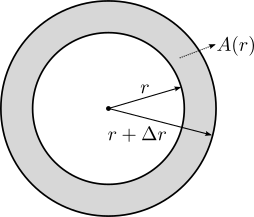
\includegraphics[width=6cm]{./area.pdf}
\end{center}
Vemos que $A(r)=\pi (r+\Delta r)^2 - \pi r^2 \approx 2\pi r\Delta r$.
De este modo, el número de partículas esperado, en media, seria de 
$n(r)=2\pi r\Delta r\rho$, si no hubiese interacciones. 

Las interacciones hacen con que el número de partículas en cada
distancia sea diferente de una distribución homogénea. Si hay
interacciones favorables, por ejemplo, la probabilidad de encontrar dos
partículas próximas es mayor. Esta distribución de partículas es uno de
los parámetros estructurales más importantes.

El programa {\tt bin/gr} calcula, a partir de la trayectoria, la función
$g(r)=n'(r)/n(r)$, done $n(r)$ esta definido anteriormente, y $n'(r)$ es
el número medio de partículas efectivamente observado entre $r$ y $r+\Delta r$
en la simulación. 

Haga una simulación de dinámica molecular con el termostato de Langevin,
ahora por más tiempo, 
usando el comando 
\command{./bin/md-langevin 15000}
Use los parámetros
$\lambda=0.01$ y $\Delta t=0.05$. Observe la trayectoria resultante y
calcule al función $g(r)$ simplemente ejecutando el programa {\tt
bin/gr}. En seguida, visualice el $g(r)$ con
\command{xmgrace gr.dat} 
Mantenga este gráfico abierto, para comparación futura. Entienda que
significa, en función de la visualización de la simulación. 

En seguida, haga una simulación de 200.000 pasos de Monte-Carlo con el programa 
{\tt bin/mc} usando una perturbación de 0.05~\AA. Observe la trayectoria
generada. Ejecute nuevamente el
programa {\tt bin/gr} para obtener la $g(r)$ de esta simulación de
Monte-Carlo. Incorpore los datos al mismo gráfico del $g(r)$ obtenido
por dinámica molecular. Compare. Las simulaciones, con sus naturalezas
totalmente distintas, muestrearon las mismas estructuras?  

\end{document}



















